%  !TeX  root  =  user_guide.tex 

\section{GDAL Tools Plugin}\label{label_plugingdaltools}

% when the revision of a section has been finalized, 
% comment out the following line:
% \updatedisclaimer

\subsection{What is GDALTools?}\label{whatsgdal}
The GDAL Tools plugin offers a GUI to the collection of tools in the Geospatial Data Abstraction Library, \url{http://gdal.osgeo.org}. These are raster management tools to query, re-project, warp, merge a wide variety of raster formats. Also included are tools to create a contour (vector) layer, or a shaded relief from a raster DEM, and to make a vrt (Virtual Raster Tile in XML format) from a collection of one or more raster files. These tools are available when the plugin is installed and activated.
\subsection{The GDAL Library}\label{gdal_lib}
The GDAL library consists of a set of command line programs, each with a large list of options. Users comfortable with running commands from a terminal may prefer the command line, with access to the full set of options. The GDALTools plugin offers an easy interface to the tools, exposing only the most popular options. 

{\setlength{\extrarowheight}{15pt}
\begin{longtable}{|p{3cm}|p{13cm}|}
\caption{List of GDAL tools}\label{tab:gdaltools} \\
\hline
Build Virtual Raster & This program builds a VRT (Virtual Dataset) that is a mosaic of the list of input gdal datasets. \\
\hline Contour & This program generates a vector contour file from the input raster elevation model (DEM).\\
\hline Rasterize &  This program burns vector geometries (points, lines and polygons) into the raster band(s) of a raster image. Vectors are read from OGR supported vector formats. Note that the vector data must in the same coordinate system as the raster data; on the fly reprojection is not provided.\\
\hline Polygonize & This utility creates vector polygons for all connected regions of pixels in the raster sharing a common pixel value. Each polygon is created with an attribute indicating the pixel value of that polygon.
The utility will create the output vector datasource if it does not already exist, defaulting to ESRI shapefile format.\\
\hline Merge &  This utility will automatically mosaic a set of images. All the images must be in the same coordinate system and have a matching number of bands, but they may be overlapping, and at different resolutions. In areas of overlap, the last image will be copied over earlier ones. \\
\hline Sieve & The gdal\_sieve.py script removes raster polygons smaller than a provided threshold size (in pixels) and replaces replaces them with the pixel value of the largest neighbour polygon. The result can be written back to the existing raster band, or copied into a new file.\\
\hline Proximity & The gdal\_proximity.py script generates a raster proximity map indicating the distance from the center of each pixel to the center of the nearest pixel identified as a target pixel. Target pixels are those in the source raster for which the raster pixel value is in the set of target pixel values.\\
\hline Near Black & This utility will scan an image and try to set all pixels that are nearly black (or nearly white) around the collar to exactly black (or white). This is often used to "fix up" lossy compressed airphotos so that color pixels can be treated as transparent when mosaicing.\\
\hline Warp & The gdalwarp utility is an image mosaicing, reprojection and warping utility. The program can reproject to any supported projection, and can also apply GCPs stored with the image if the image is "raw" with control information. \\
\hline Grid & This program creates regular grid (raster) from the scattered data read from the OGR datasource. Input data will be interpolated to fill grid nodes with values, you can choose from various interpolation methods.\\
\hline Translate & The gdal\_translate utility can be used to convert raster data between different formats, potentially performing some operations like subsettings, resampling, and rescaling pixels in the process.\\
\hline Information & The gdalinfo program lists various information about a GDAL supported raster dataset. \\
\hline Assign Projection &  The gdalwarp utility is an image mosaicing, reprojection and warping utility. The program can reproject to any supported projection, and can also apply GCPs stored with the image if the image is "raw" with control information.
-s\_srs srs def:
source spatial reference set. The coordinate systems that can be passed are anything supported by the OGRSpatialReference.SetFromUserInput() call, which includes EPSG PCS and GCSes (ie. EPSG:4296), PROJ.4 declarations (as above), or the name of a .prf file containing well known text. 
-t\_srs srs\_def:
target spatial reference set. The coordinate systems that can be passed are anything supported by the OGRSpatialReference.SetFromUserInput() call, which includes EPSG PCS and GCSes (ie. EPSG:4296), PROJ.4 declarations (as above), or the name of a .prf file containing well known text. \\
\hline Build Overviews &  The gdaladdo utility can be used to build or rebuild overview images for most supported file formats with one over several downsampling algorithms.\\
\hline Clipper & This utility will automatically mosaic a set of images. All the images must be in the same coordinate system and have a matching number of bands, but they may be overlapping, and at different resolutions. In areas of overlap, the last image will be copied over earlier ones. 
-ul\_lr ulx uly lrx lry:
The extents of the output file. If not specified the aggregate extents of all input files will be used. \\
\hline RGB to PCT &  This utility will compute an optimal pseudo-color table for a given RGB image using a median cut algorithm on a downsampled RGB histogram. Then it converts the image into a pseudo-colored image using the color table. This conversion utilizes Floyd-Steinberg dithering (error diffusion) to maximize output image visual quality. \\
\hline PCT to RGB &  This utility will convert a pseudocolor band on the input file into an output RGB file of the desired format.\\
\hline
\end{longtable}

\begin{figure}[ht]
   \centering
   \caption{The \emph{GDALTools} menu list \nixcaption}\label{gdaltools_menu}
   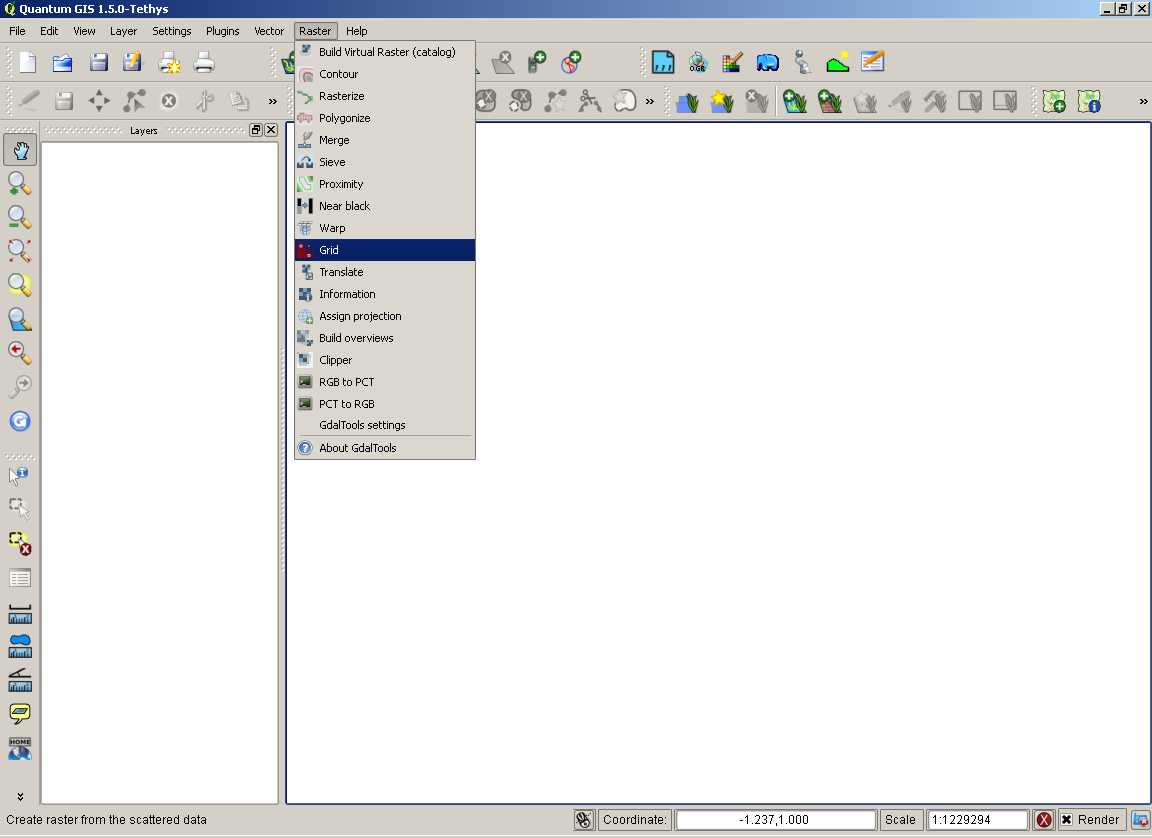
\includegraphics[clip=true, width=12cm]{plugins_gdaltools_images/raster_menu}
\end{figure}

\subsection{Examples}\label{gdal_examples}
Below are some examples of use of the tools.
\subsubsection{Getting information about a raster}
\begin{figure}[ht]
   \centering
   \caption{The \emph{Information} dialog window \nixcaption}\label{gdalinfo}
   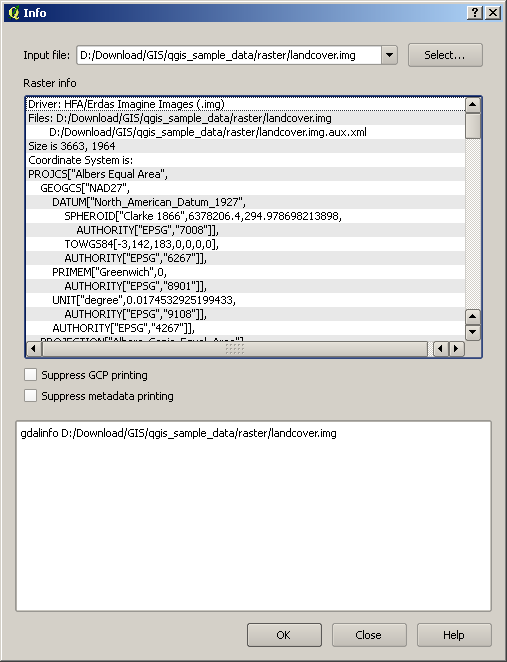
\includegraphics[clip=true, width=12cm]{plugins_gdaltools_images/gdalinfo}
\end{figure}

\subsubsection{Creating contour lines}
This example will create contour lines from an SRTM elevation tile.
\begin{figure}[ht]
   \centering
   \caption{The \emph{Contours} dialog window \nixcaption}\label{gdal_contour}
   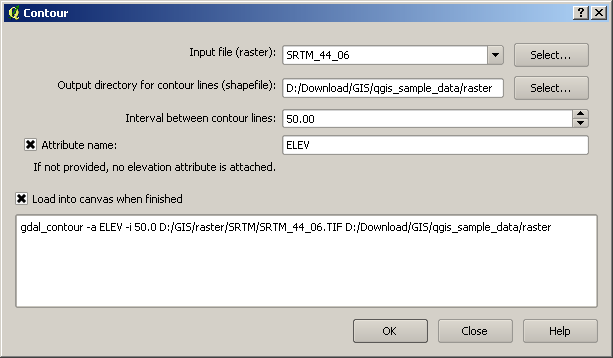
\includegraphics[clip=true, width=12cm]{plugins_gdaltools_images/gdal_contour}
\end{figure}
and the result:
\begin{figure}[ht]
   \centering
   \caption{The resulting contours layer \nixcaption}\label{gdal_contour}
   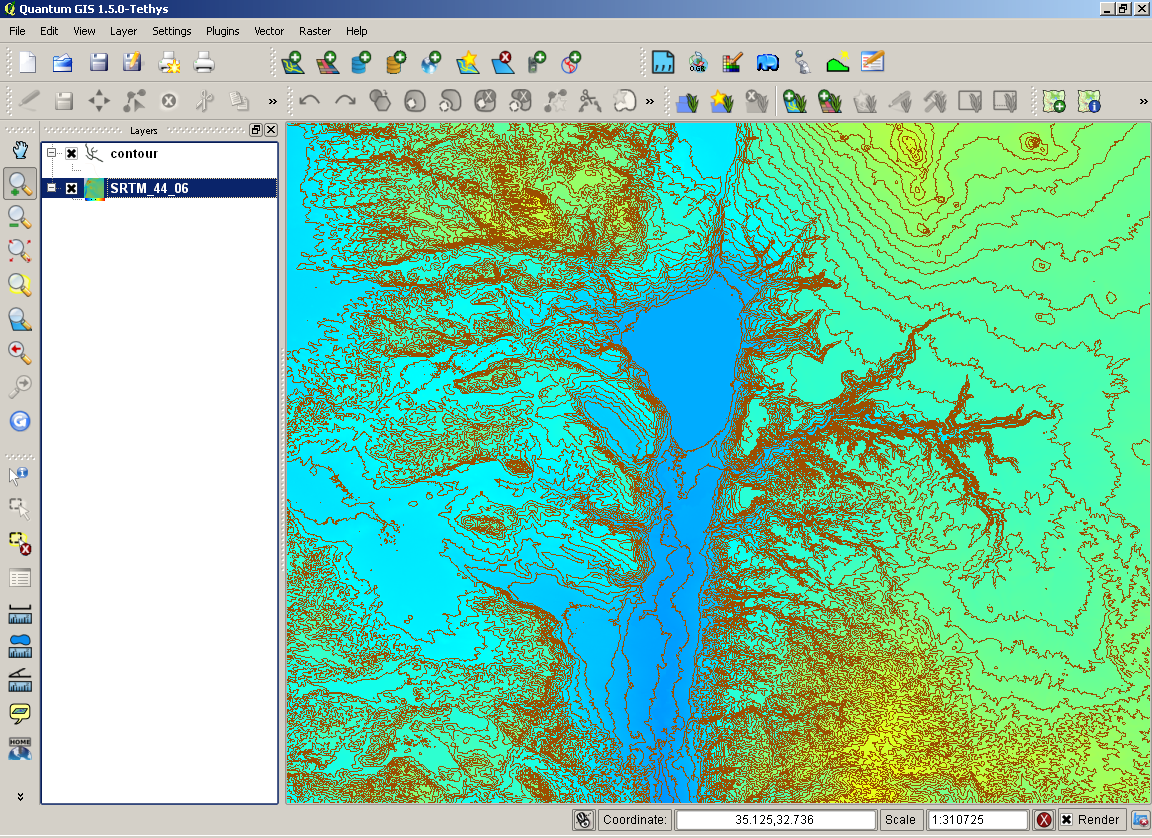
\includegraphics[clip=true, width=12cm]{plugins_gdaltools_images/qgis_contours}
\end{figure}

\subsubsection{Using GDALwarp to reproject a raster}
Here's the dialog window for reprojecting a landcover image, originally in the Albers Equal Area projection for Alaska (from the QGIS sample dataset) into Lon/Lat WGS84 (EPSG:4326).
\begin{figure}[ht]
   \centering
   \caption{The \emph{GDAL warp} dialog window \nixcaption}\label{gdalwarp}
   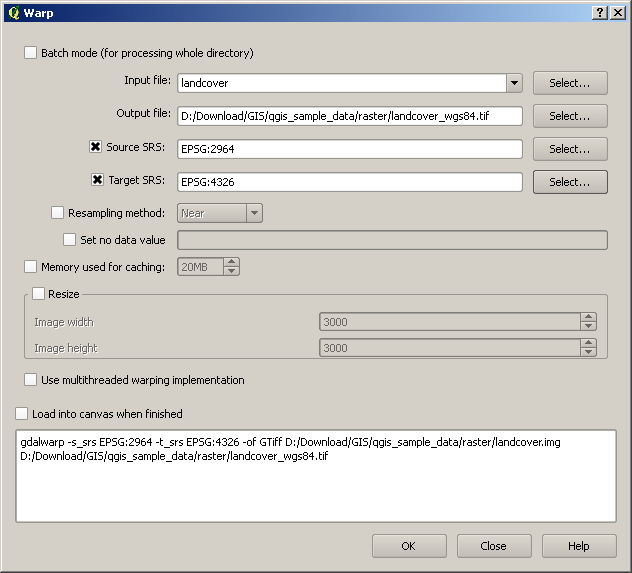
\includegraphics[clip=true, width=12cm]{plugins_gdaltools_images/gdalwarp}
\end{figure}

\FloatBarrier
